\documentclass{beamer}
\setbeamertemplate{navigation symbols}{}
\usepackage{comment}

\setbeamercolor{frametitle}{fg=black,bg=white}
\setbeamercolor{title}{fg=black,bg=yellow!85!orange}
\usetheme{AnnArbor}

\usepackage{textpos} % package for the positioning
\usepackage{listings}
\usepackage{xcolor}
\usepackage[most]{tcolorbox}
\usepackage{mathtools}
\usepackage{graphicx}
\usepackage{graphbox}
\usepackage{caption}
\DeclareCaptionType{code}[Code Listing][List of Code Listings] 

\definecolor{codegreen}{rgb}{0,0.6,0}
\definecolor{codegray}{rgb}{0.5,0.5,0.5}
\definecolor{codepurple}{rgb}{0.58,0,0.82}
\definecolor{backcolour}{rgb}{0.95,0.95,0.92} 
\lstdefinestyle{mystyle}{
    backgroundcolor=\color{backcolour},   
    commentstyle=\color{codegreen},
    keywordstyle=\color{magenta},
    numberstyle=\tiny\color{codegray},
    stringstyle=\color{codepurple},
    basicstyle=\ttfamily\footnotesize,
    breakatwhitespace=false,         
    breaklines=true,                 
    captionpos=b,                    
    keepspaces=true,                 
    numbers=left,                    
    numbersep=5pt,                  
    showspaces=false,                
    showstringspaces=false,
    showtabs=false,                  
    tabsize=2
}

\lstset{style=mystyle}

\lstdefinelanguage
   [x64]{Assembler}     % add a "x64" dialect of Assembler
   [x86masm]{Assembler} % based on the "x86masm" dialect
   % with these extra keywords:
   {morekeywords={CDQE,CQO,CMPSQ,CMPXCHG16B,JRCXZ,LODSQ,MOVSXD, %
                  POPFQ,PUSHFQ,SCASQ,STOSQ,IRETQ,RDTSCP,SWAPGS, %
                  rax,rdx,rcx,rbx,rsi,rdi,rsp,rbp, %
                  r8,r8d,r8w,r8b,r9,r9d,r9w,r9b, %
                  r10,r10d,r10w,r10b,r11,r11d,r11w,r11b, %
                  r12,r12d,r12w,r12b,r13,r13d,r13w,r13b, %
                  r14,r14d,r14w,r14b,r15,r15d,r15w,r15b}} %


\beamersetuncovermixins{\opaqueness<1>{25}}{\opaqueness<2->{15}}

%Copyright
\addtobeamertemplate{frametitle}{}{%
\begin{textblock*}{50mm}(0cm,-1.25cm)
\color{yellow!85!orange}
\tiny{Copyright \copyright 2024 CNM.}
\end{textblock*}}

% position the logo
\addtobeamertemplate{frametitle}{}{%
\begin{textblock*}{100mm}(11.4cm,-1.3cm)

\includegraphics[height=1cm,width=1cm,keepaspectratio]{fig/ddclogotransparent.png}
\end{textblock*}}

\AtBeginSection[]{
  \begin{frame}
  \vfill
  \centering
  \begin{beamercolorbox}[sep=8pt,center,shadow=true,rounded=true]{title}
    \usebeamerfont{title}\insertsectionhead\par%
  \end{beamercolorbox}
  \vfill
  \end{frame}
}

\begin{document}
\title{Quantum Math}
\author{Brian Rashap}
\date{August 2025} 



\begin{frame}
\titlepage
\end{frame}

\section{Algebra}
\begin{frame}\frametitle{Algebra Overview}
\begin{itemize}
\item Functions
\item Transformations
\item Polynomials
\item Rational Functions
\item Exponentials and Logarithms
\end{itemize}
\end{frame}

\begin{frame}\frametitle{Cartesian Coordinates}
\begin{columns}
\begin{column}{4cm}
Some text
\end{column}
\begin{column}{6cm}
\begin{center}
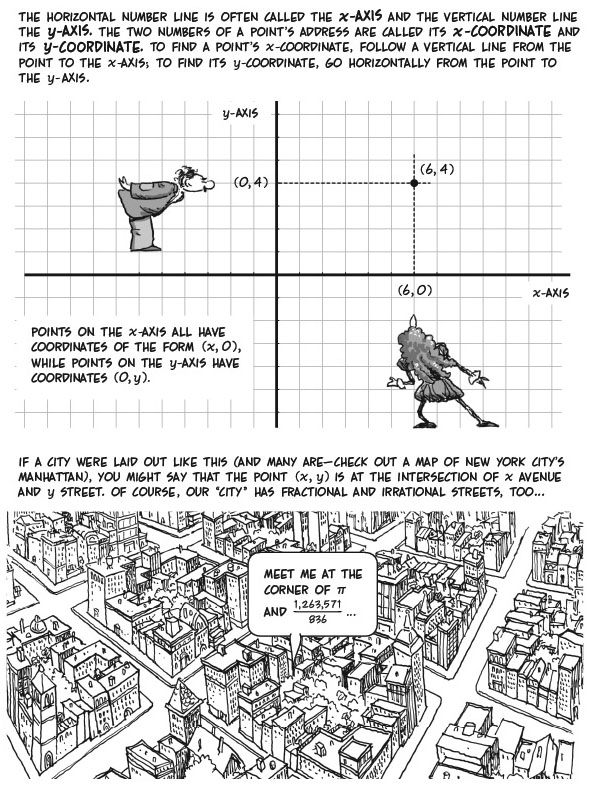
\includegraphics[height=7.5cm]{fig/plotting.jpg}
\end{center}
\end{column}
\end{columns}
\end{frame}

\begin{frame}\frametitle{Measuring Distance - Pythagorean Theorem}
\begin{columns}
\begin{column}{6cm}
Pythagorean Theorem:
\begin{center}
$a^2 + b^2 = c^2$
\end{center}

For example: \newline

\hspace*{10mm}$d^2 = 3^2 + 4^2$ \newline
\hspace*{10mm}$d^2 = 9 + 16 = 25$ \newline
\hspace*{10mm}$d = \sqrt{25} = 5$ \newline

More generally for two points $P(x_1,y_1)$ and $Q(x_2,y_2)$ \newline

\hspace*{10mm}$d^2 = (x_2-x_1)^2 + (y_2 - y_1)^2$ \newline
\hspace*{10mm}$d = \sqrt{(x_2-x_1)^2 + (y_2 - y_1)^2}$ \newline

Noting that $\mid a \mid = (a)^2$: \newline


\end{column}
\begin{column}{5cm}
\begin{center}
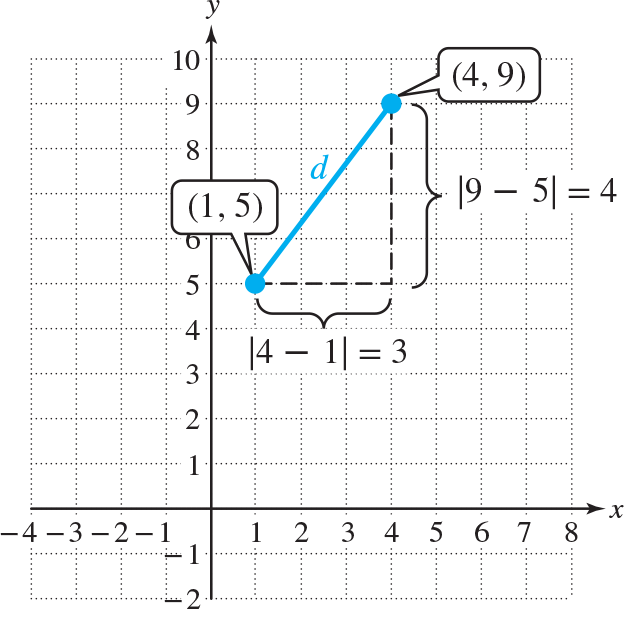
\includegraphics[width=4cm]{fig/pythag.png}
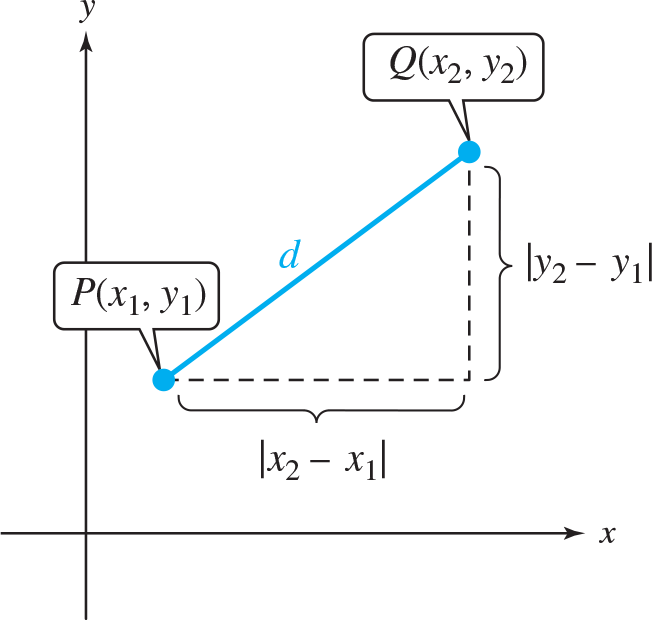
\includegraphics[width=4cm]{fig/pythag2.png}
\end{center}
\end{column}
\end{columns}
\end{frame}

\begin{frame}\frametitle{Midpoints and Intercepts}
\begin{columns}
\begin{column}{6cm}

Midpoint: \newline

\hspace*{10mm}$M = (\frac{x_1+x_2}{2},\frac{y_2+y_1}{2})$ \newline


Intercepts: \newline

Two key features of a graph are where the graph intersects the x and y axes, the x-intercept and y-intercept, respectively.


\end{column}
\begin{column}{5cm}
\begin{center}
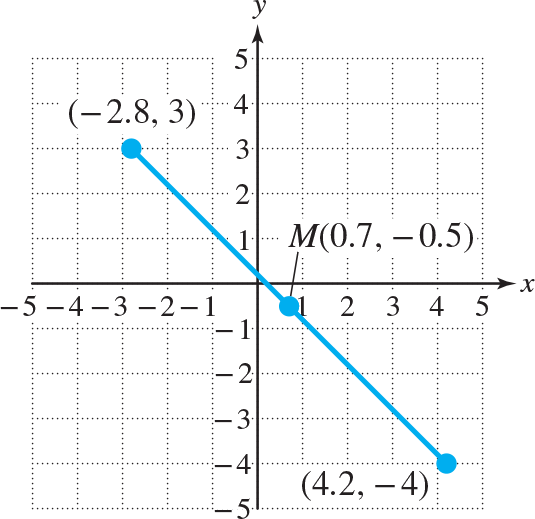
\includegraphics[width=4cm]{fig/midpoint.png}
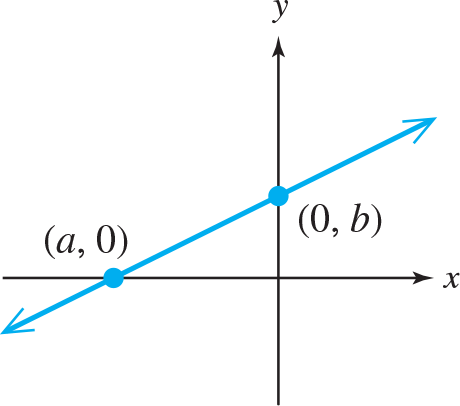
\includegraphics[width=4cm]{fig/intercept.png}
\end{center}
\end{column}
\end{columns}
\end{frame}


\begin{frame}\frametitle{The Circle}
\begin{columns}
\begin{column}{7.5cm}

A circle is a set of all points that are equidistant from a fixed point called the center $(h,k)$. The distance from any point on the cirecle to the center is called the radius ($r$)

$r = \sqrt{(x-h)^2 + (y-k)^2}$ \newline

Equation of a circle: \newline
Standard form: $(x-h)^2 + (y-k)^2 = r^2$ \newline

Expand binomials: $x^2-hx+h^2+y^2-ky+k^2 - r^2 = 0$ \newline

General form: $x^2+y^2-hx-ky+(h^2+k^2-r^2)=0$

\hspace*{10mm} or

$x^2 + y^2 + Ax + By + C = 0$

\end{column}
\begin{column}{3.5cm}
\begin{center}
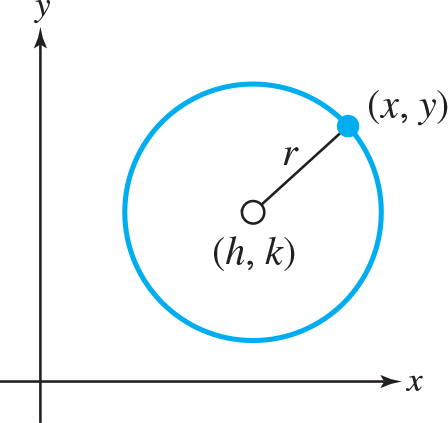
\includegraphics[width=3cm]{fig/circle.png}
\end{center}
\end{column}
\end{columns}
\end{frame}



\begin{frame}\frametitle{Domain and Range}
\begin{columns}
\begin{column}{6cm}
\begin{center}
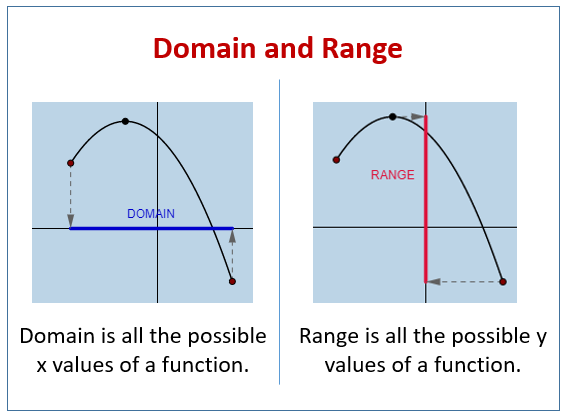
\includegraphics[width=6cm]{fig/domain-range.png}
\end{center}
\end{column}

\begin{column}{5cm}
A set of ordered pairs $(x,y)$ is called a relation in x and y. 
\begin{itemize}
\item The set of x-values in the ordered pairs is called the domain of the relations.
\item The set of y-values in the ordered pairs is called the range of the relations.
\end{itemize}
\end{column}
\end{columns}
\end{frame}


\begin{frame}\frametitle{Linear Equations with Two Variables}
A linear equation in variables $x$ and $y$ can be written in the standard form:
\begin{equation}
Ax + By = C
\end{equation}

However, it is more common to see it in slope-intercept form:
\begin{equation}
y = mx + b
\end{equation}
where, $m$ is the slope and $b$ is the y-intercept
\end{frame}

\begin{frame}\frametitle{Linear Conversion - Slope and Y-Intercept}
\begin{columns}
\begin{column}{6cm}
\begin{center}
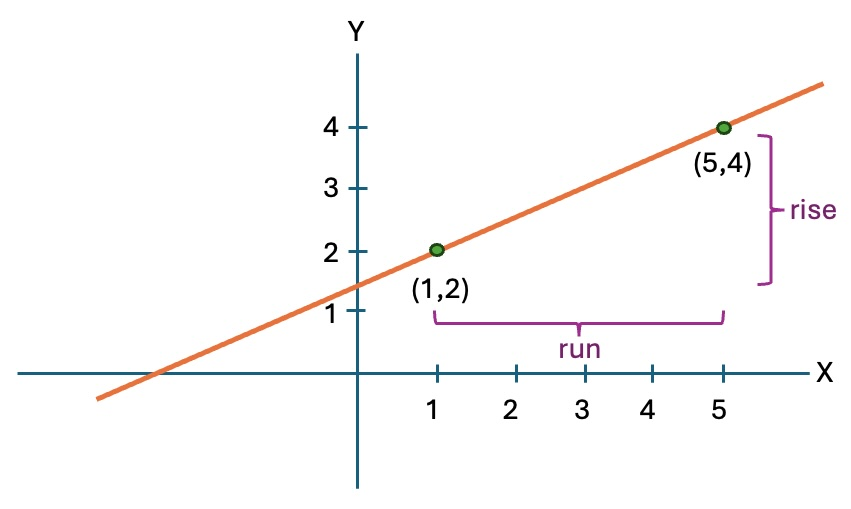
\includegraphics[width=5cm]{fig/slope.jpg}

$y = mx + b$

where $m$ is slope and $b$ y-intercept. 
\end{center}
\end{column}

\begin{column}{5.2cm}
For example, given two points:
\begin{itemize}
\item $(x_1,y_1) = (1,2)$
\item $(x_2,y_2) = (5,4)$
\end{itemize}
Find slope
\begin{itemize}
\item $m = \frac{rise}{run} = \frac{4-2}{5-1} = \frac{1}{2}$
\end{itemize}
Find y-intercept
\begin{itemize}
\item $y_1 = m * x_1 + b$
\item $b = y_1 - (m * x_1$)
\item $b = 2 - (\frac{1}{2} * 1) = 1 \frac{1}{2}$
\end{itemize}
\end{column}
\end{columns}

\vspace{1cm}

Use this to find the conversion from Celsius to Fahrenheit.
\end{frame}

\begin{frame}\frametitle{Parallel and Perpendicular Lines}
\begin{center}
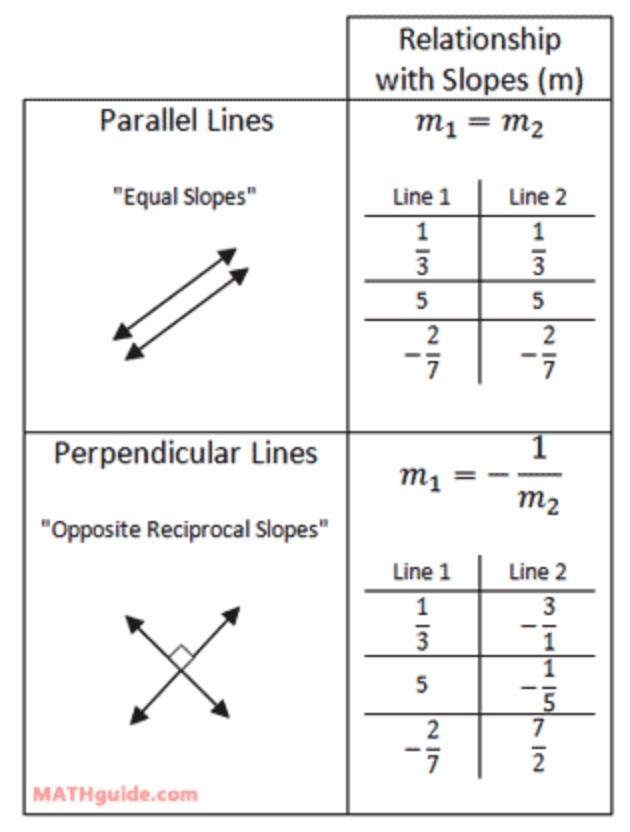
\includegraphics[width=5.5cm]{fig/parperp.jpg}
\end{center}
\end{frame}



\begin{frame}\frametitle{Linear Regression}
\begin{columns}
\begin{column}{6cm}
\begin{center}
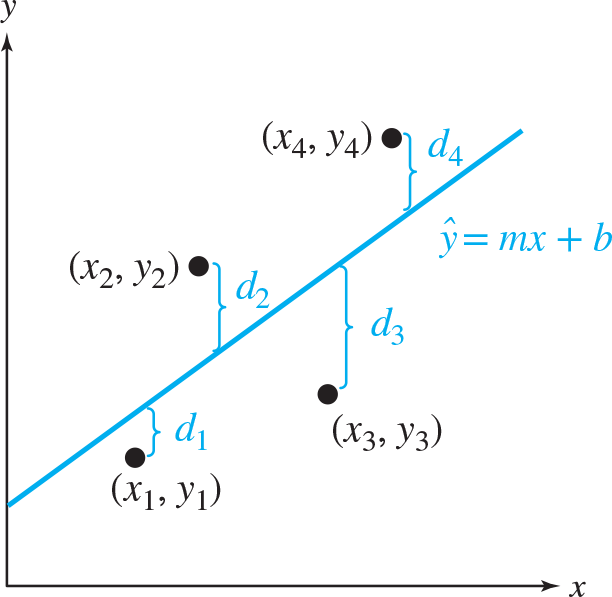
\includegraphics[width=5cm]{fig/lsqr.png}
\end{center}
\end{column}

\begin{column}{5cm}
Consider a set of data: $(x_1,y_1),(x_2,y_2),(x_3,y_3),...,(x_n,y_n)$
\begin{itemize}
\item The least-squares regression line $\hat{y} = mx + b$, is a unique line that minimizes the sum of the squared vertical deviations from the the observed data points to the line.
\end{itemize}
\end{column}
\end{columns}

\vspace{1cm}

Use this to find the conversion from Celsius to Fahrenheit.
\end{frame}


\begin{frame}\frametitle{Recognizing Functions}
\begin{columns}
\begin{column}{4.5cm}
An algebraic function provides a "y-value" for every "x-value"
\begin{itemize}
\item Linear: $y = x + 2$
\item Quadratic: $y = x^2$
\item Periodic: $y = sin(x)$
\end{itemize}
\end{column}
\begin{column}{7cm}
\begin{center}
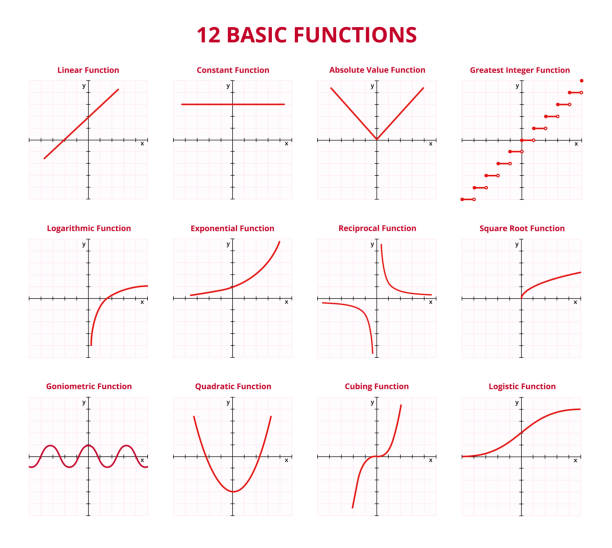
\includegraphics[width=7cm]{fig/basicfun.jpg}
\end{center}
\end{column}
\end{columns}
\end{frame}


\begin{frame}\frametitle{Vertical and Horizontal Shifts}
\begin{columns}
\begin{column}{5.0cm}
\begin{center}
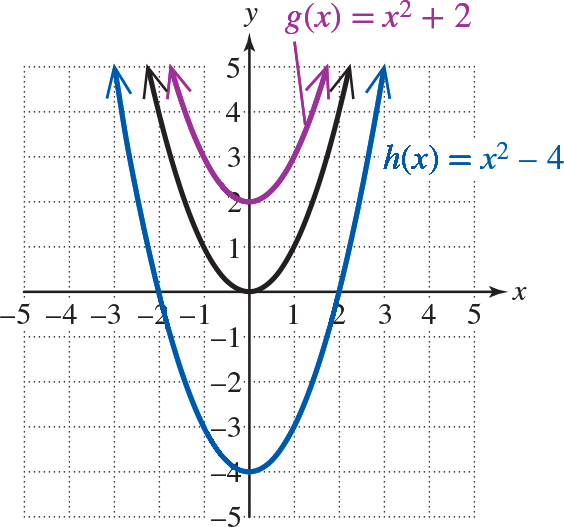
\includegraphics[height=4.5cm]{fig/shiftV.png}
\end{center}
\end{column}
\begin{column}{6.0cm}
\begin{center}
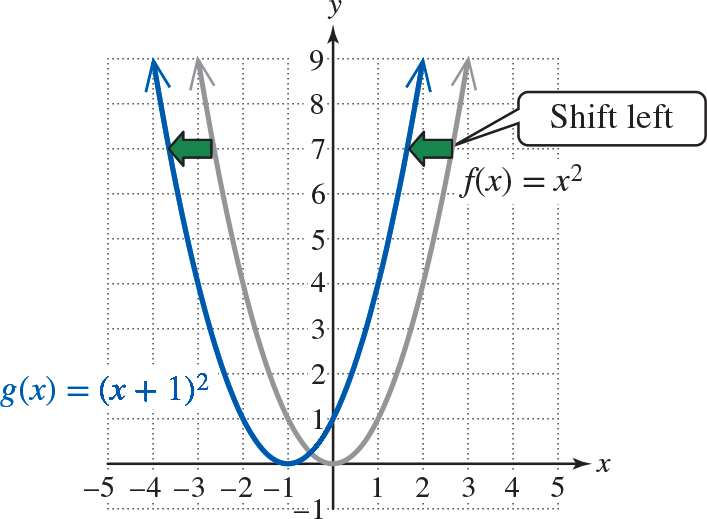
\includegraphics[height=4.5cm]{fig/shiftH.png}
\end{center}
\end{column}
\end{columns}
\end{frame}

\begin{frame}\frametitle{Shrink and Expand}

\begin{center}
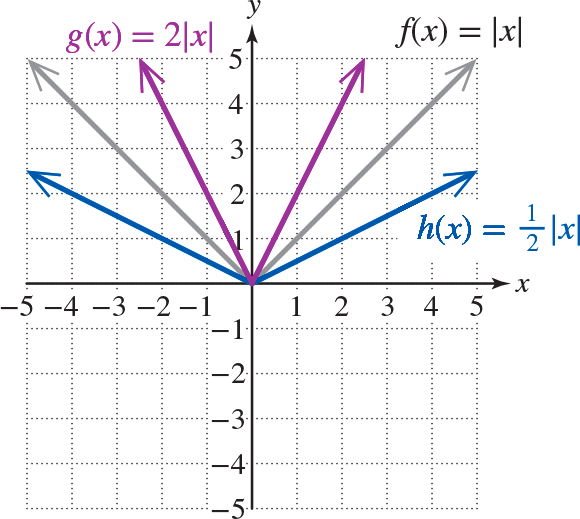
\includegraphics[height=6.0cm]{fig/stretchV.png}
\end{center}

\end{frame}


\begin{frame}\frametitle{X and Y Reflections}
\begin{columns}
\begin{column}{5.5cm}
\begin{center}
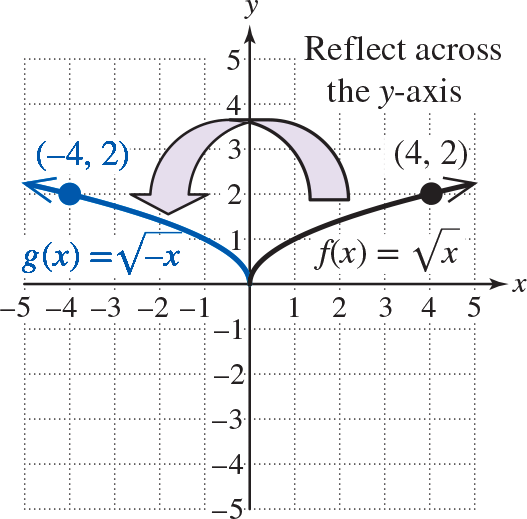
\includegraphics[height=4.5cm]{fig/reflectX.png}
\end{center}
\end{column}
\begin{column}{5.5cm}
\begin{center}
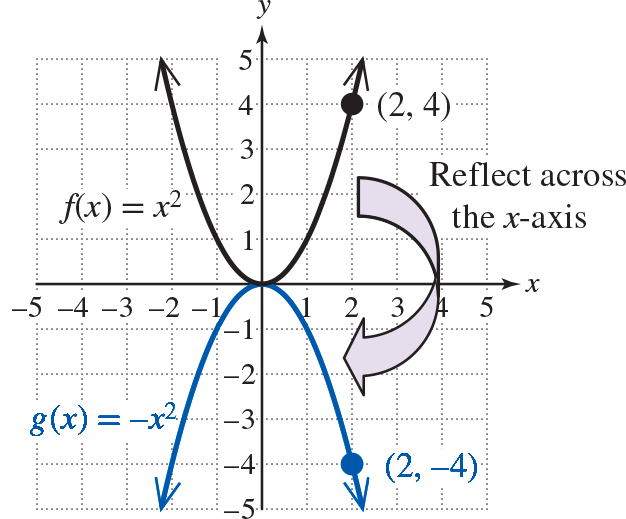
\includegraphics[height=4.5cm]{fig/reflectY.png}
\end{center}
\end{column}
\end{columns}
\end{frame}

\begin{frame}\frametitle{Summary - Transformations of Functions}
\begin{center}
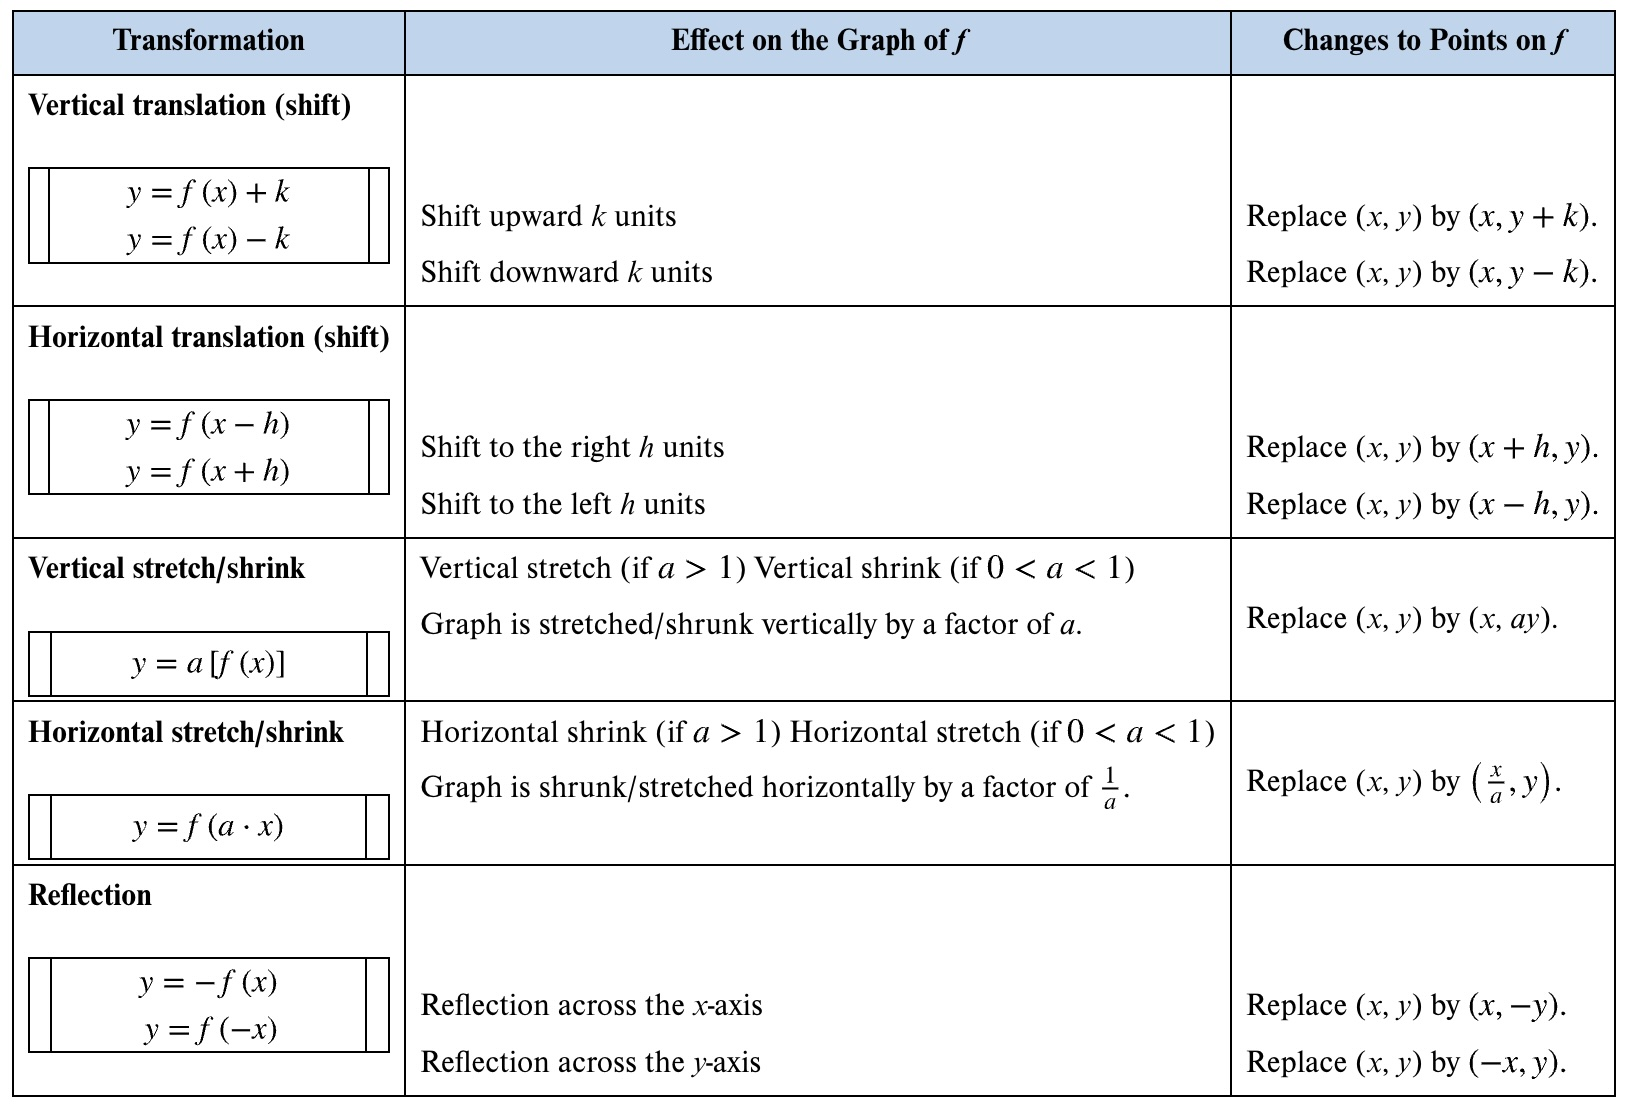
\includegraphics[width=10cm]{fig/transform.jpg}
\end{center}
\end{frame}


\begin{frame}\frametitle{Piece-Wise Functions}
\begin{columns}
\begin{column}{6cm}
\begin{center}
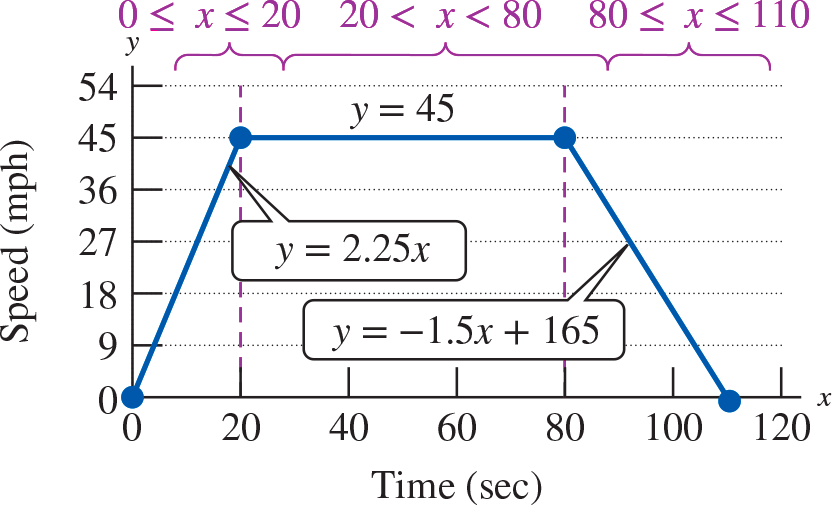
\includegraphics[width=6cm]{fig/pwfunct1.png}
\end{center}
\end{column}
\begin{column}{5cm}
\begin{center}
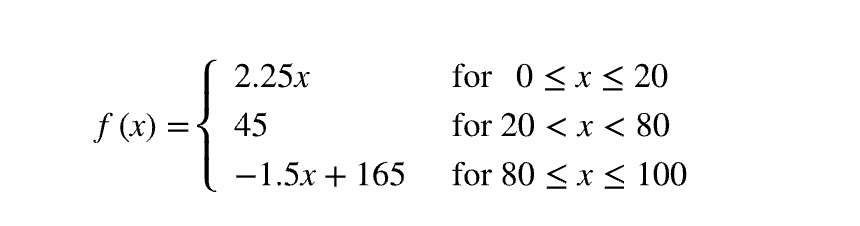
\includegraphics[width=6cm]{fig/pwfunct2.jpg}
\end{center}
\end{column}
\end{columns}
\end{frame}

\begin{frame}\frametitle{Rate of Change}
Given points $(x_1,y_1)$ and $(x_2,y_2)$ as points on the graph of a function $f()$, if $f()$ is defined on the interval $[x_1,x_2]$, then the average rate of change is the slope of the secant\footnote{Secante comes from the latin secare meaning "to cut."} line containing $(x_1,f(x_1))$ and $(x_2,f(x_2))$. 

\begin{center}
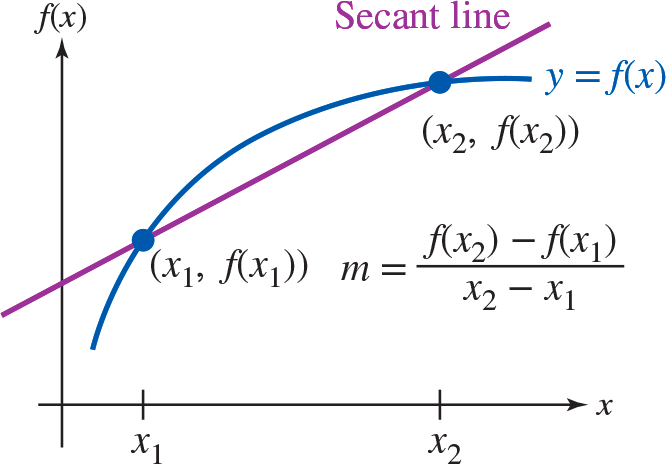
\includegraphics[width=6cm]{fig/roc.png}
\end{center}
\end{frame}


\begin{frame}\frametitle{Difference Quotient}
Suppose we choose a value $x$ from the domain of $f()$ and a second value $x + h$, where $h \neq 0$, but very small.

\begin{center}
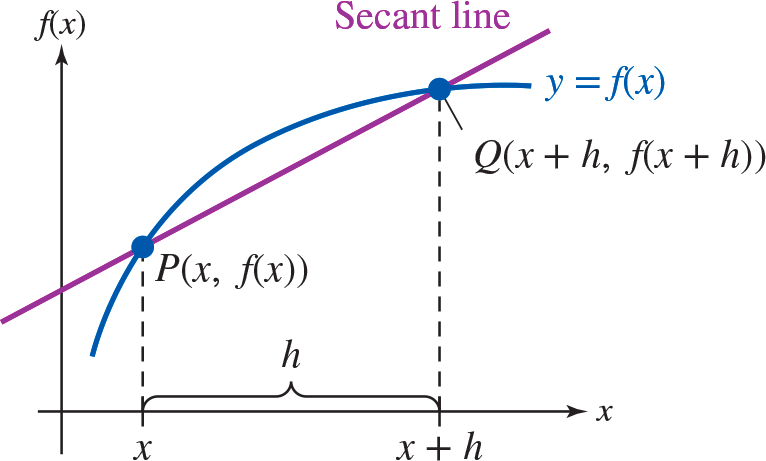
\includegraphics[width=5cm]{fig/roc2.png}
\end{center}

The difference quotient\footnote{The difference quotient is important to calculus, where the exact rate of change at a point is given by $ \lim_{h \rightarrow 0}(m) $}.
\begin{equation}
m = \frac{f(x+h) - f(x)}{(x+h) - x} = \frac{f(x+h) - f(x)}{h}
\end{equation}

\end{frame}

\begin{frame}\frametitle{Increaing, Decreaing, Constant}
\begin{center}
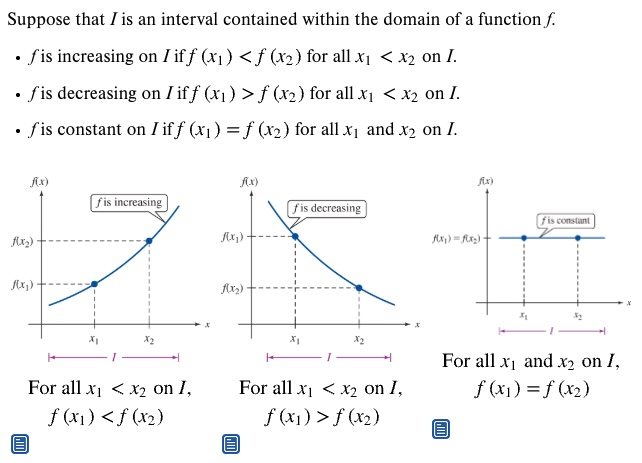
\includegraphics[height=8cm]{fig/idc.jpg}
\end{center}
\end{frame}

\begin{frame}\frametitle{Local Minima and Maxima}

\begin{itemize}
\item $f(a)$ is a relative maximum of $f$ if there exists an open interval\footnote{An open interval is an interval in which the endpoints are not included.} containing a such that $f(a) \geq f(x)$ for all $x$ in the interval.
\item $f(b)$ is a relative minimum of $f$ if there exists an open interval\footnote{An open interval is an interval in which the endpoints are not included.} containing a such that $f(b) \leq f(x)$ for all $x$ in the interval.
\end{itemize}
\begin{center}
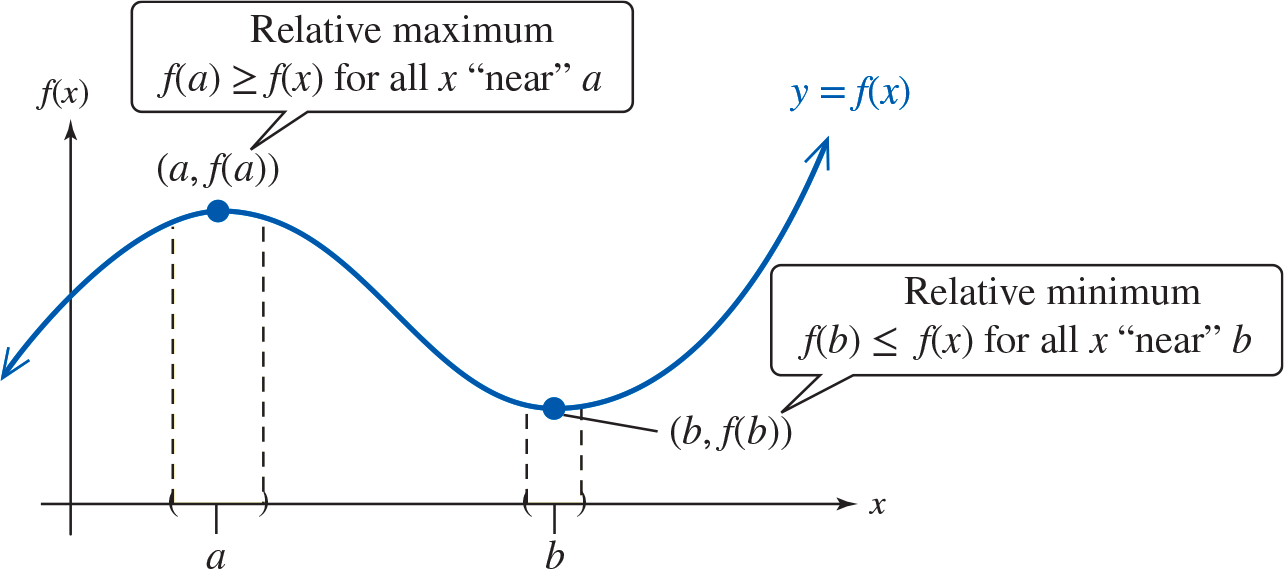
\includegraphics[width=8cm]{fig/minmax.png}
\end{center}
\end{frame}


\begin{frame}\frametitle{Operations on Functions}

\end{frame}


\begin{frame}\frametitle{Exponential Functions}
\begin{itemize}
\item Linear growth - a constant rate of change, that is,a constant number by which the output increased for each unit increase in input.
\item Exponential growth - increase based on a constant multiplicative rate of change over equal increments of time, that is, a percent increase of the original amount over time.
\end{itemize}

\begin{center}
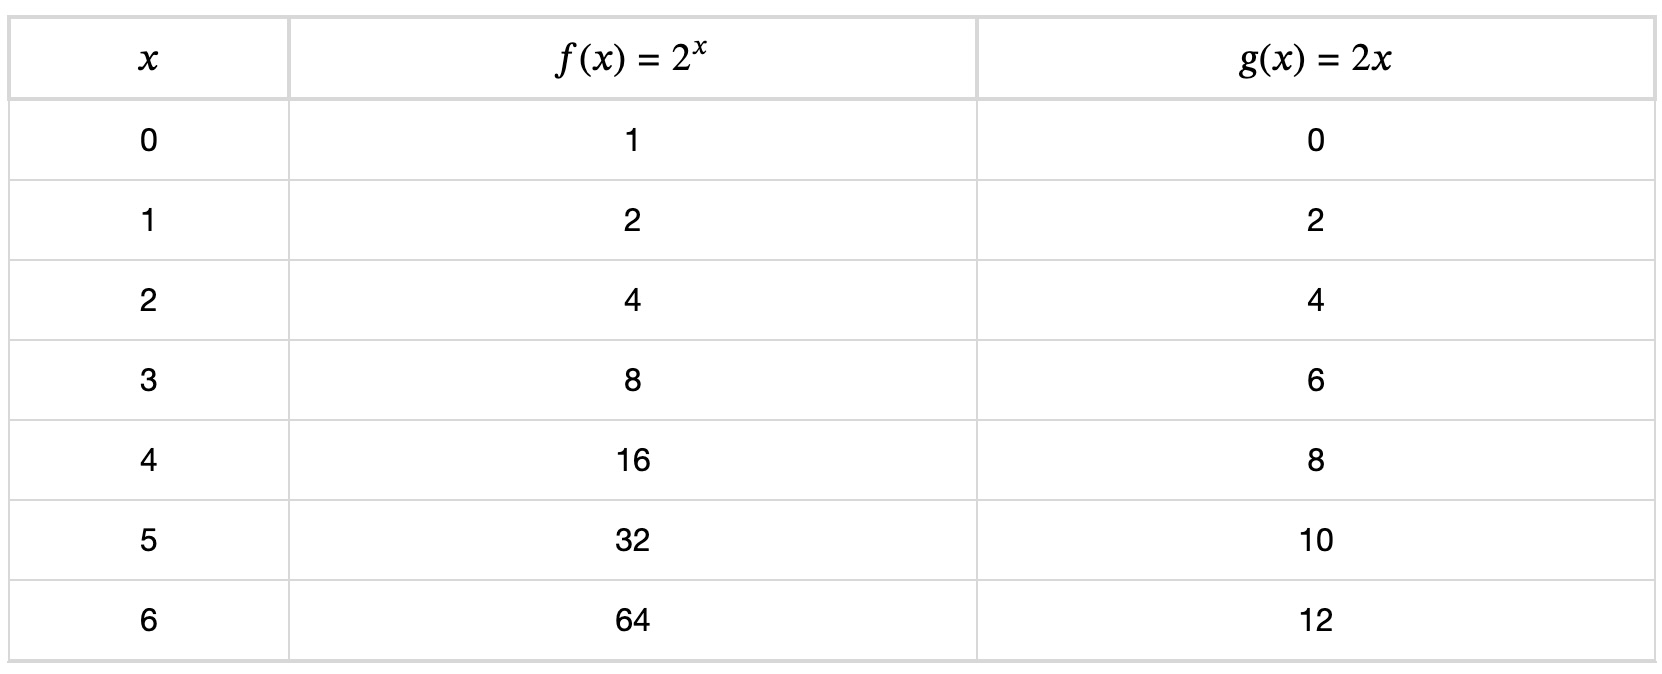
\includegraphics[width=12cm]{fig/exp_growth.jpg}
\end{center}

\end{frame}


\begin{frame}\frametitle{Origami to the Moon}
\begin{center}
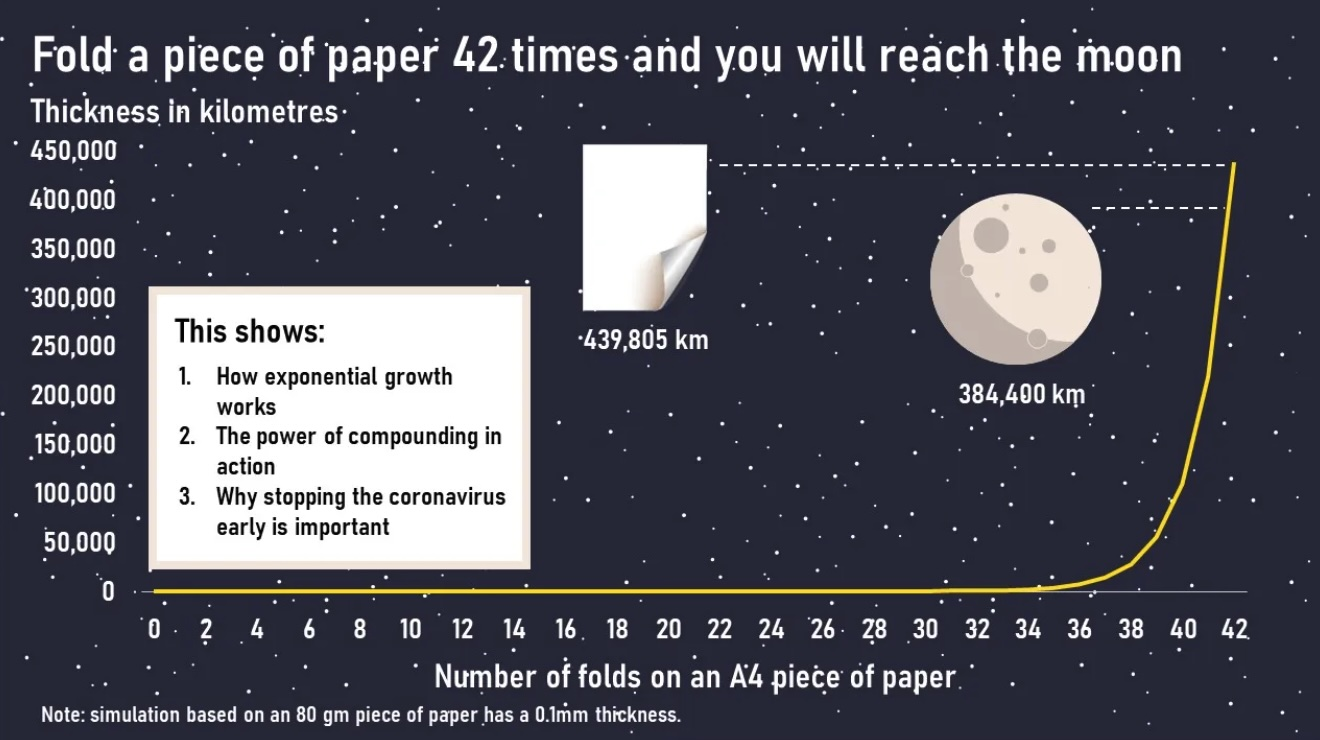
\includegraphics[width=12cm]{fig/40fold.jpg}
\end{center}
\end{frame}

\begin{frame}\frametitle{What about Negative Exponents}
\begin{columns}
\begin{column}{7cm}
The general form of an exponential function is $f(x) = ab^x$, where $a$ is any non-zero number and $b$ is an positive number not equal to 1.

\begin{itemize}
\item If $b > 1$ the function grows at a rate proportional to its size.
\item If $0 < b < 1$ the function decays at a rate proportional to its size.
\end{itemize}
\end{column}

\begin{column}{5cm}
For example, $f(x) = 2^x$:
\begin{center}
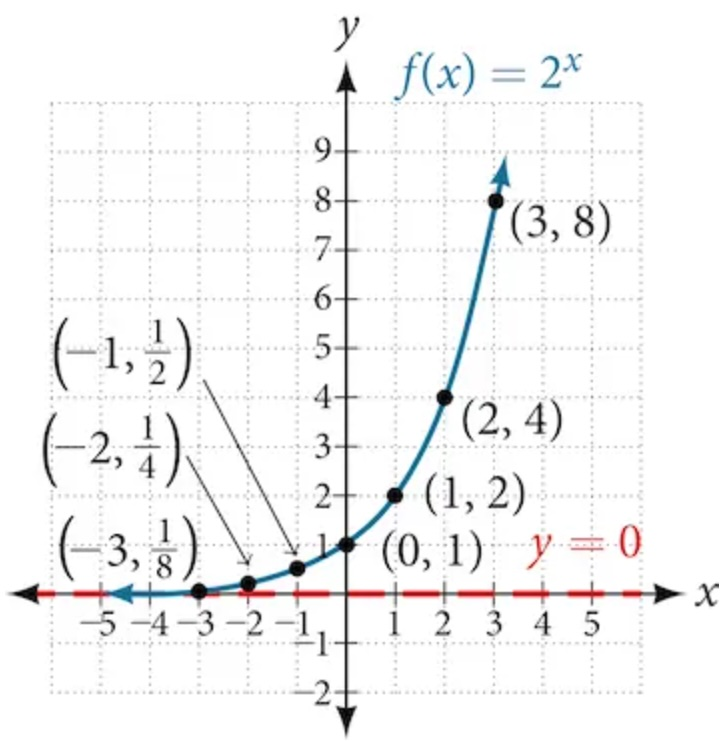
\includegraphics[width=4cm]{fig/exp2g.jpg}
\end{center}
\end{column}
\end{columns}

\begin{center}
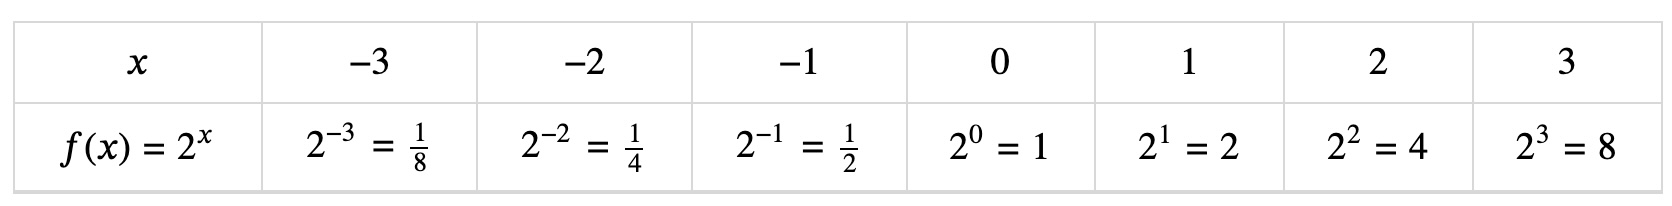
\includegraphics[width=12cm]{fig/exp2t.jpg}
\end{center}
\end{frame}

\begin{frame}\frametitle{Scientific (SI) Prefixes}
\begin{center}
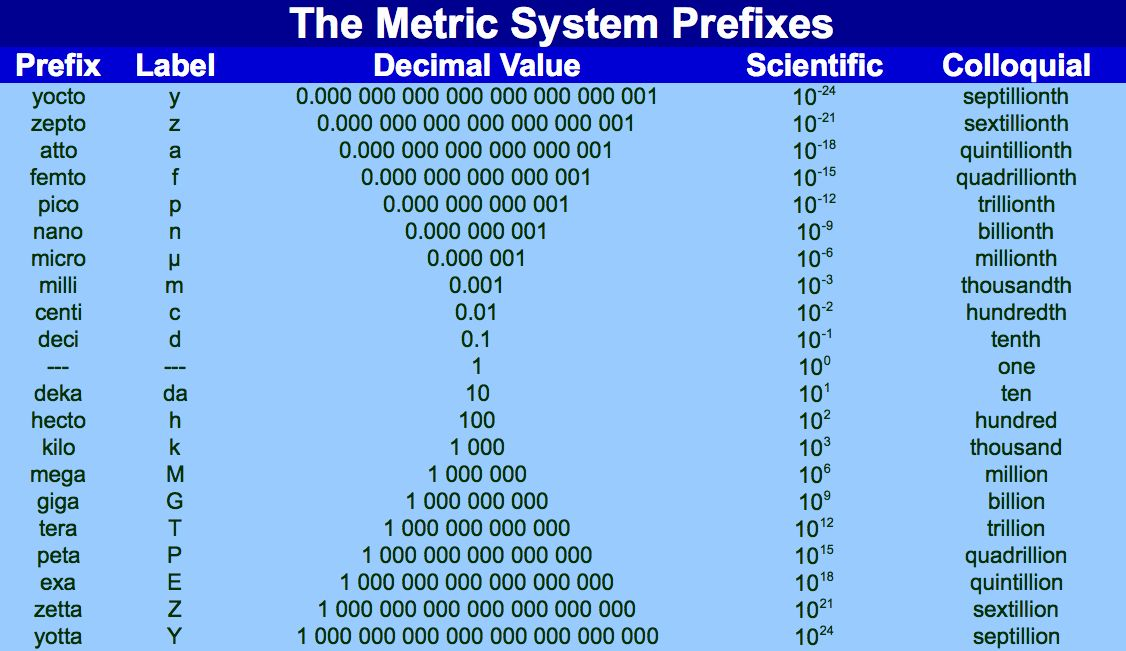
\includegraphics[width=12cm]{fig/si_prefixes.jpg}
\end{center}
\end{frame}

\begin{frame}\frametitle{$e$ - an interesting aside}
The letter e represents the irrational number:
\begin{equation}
e = (1 + \frac{1}{n})^n
\end{equation}
as $n$ increases without bound. \newline



The number $e$ is used as a base for many real-world exponential models. To work with base e, we use the approximation,  $e \approx 2.718282$. The constant was named by the Swiss mathematician Leonhard Euler (1707–1783) who first investigated and discovered many of its properties.
\end{frame}


\begin{frame}\frametitle{Graphing Exponentials}
\begin{columns}
\begin{column}{7cm}

Shifts:
\begin{center}
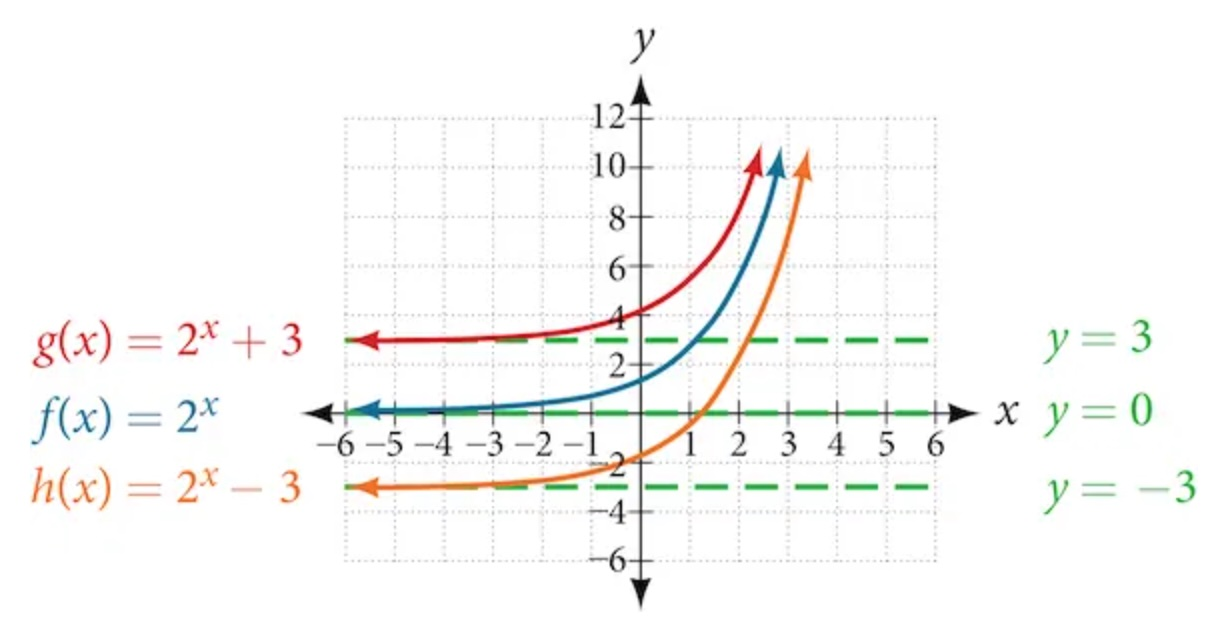
\includegraphics[width=6.5cm]{fig/exp2vert.jpg}
\end{center}

\begin{center}
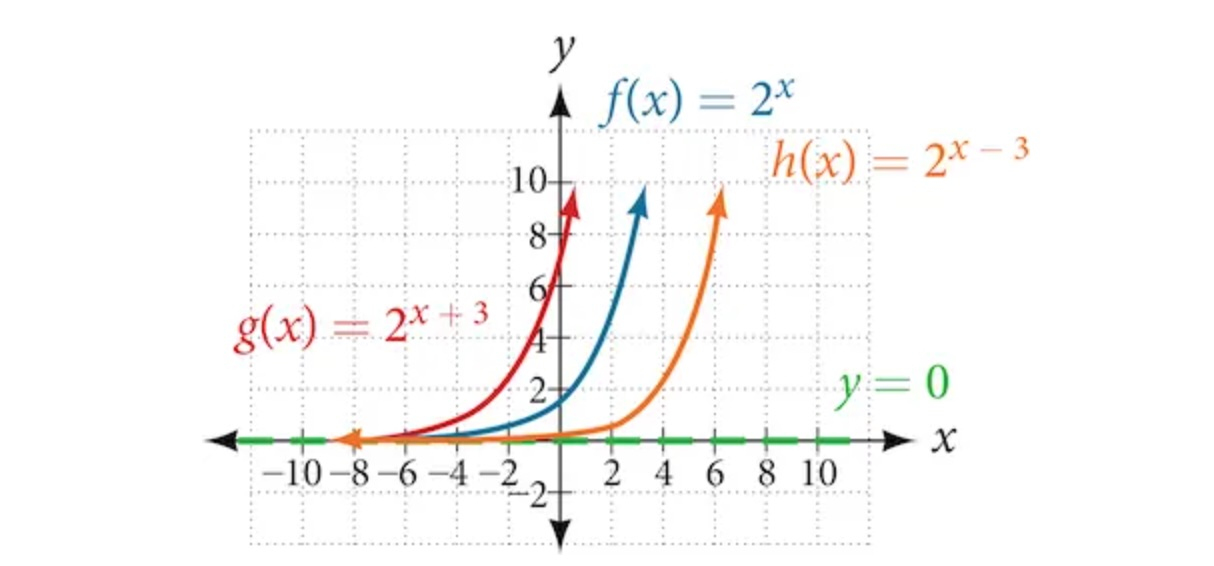
\includegraphics[width=6.5cm]{fig/exp2hor.jpg}
\end{center}

\end{column}

\begin{column}{5cm}
Stretch:
\begin{center}
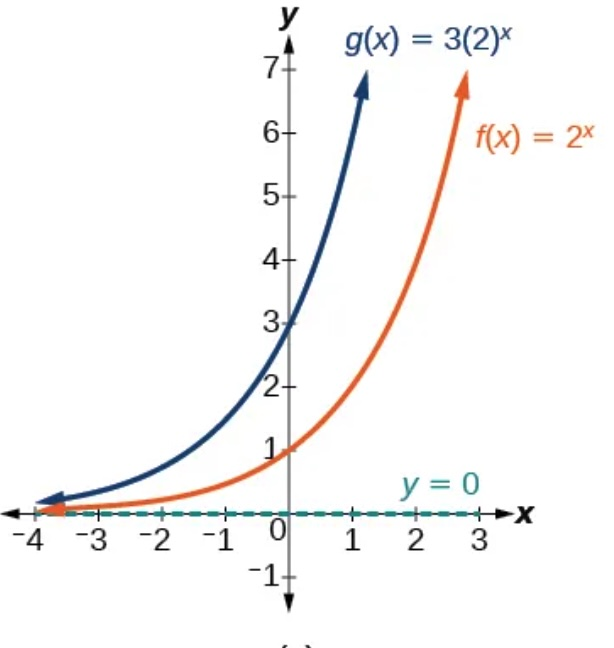
\includegraphics[width=2.8cm]{fig/exp2v.jpg}
\end{center}

Flip:
\begin{center}
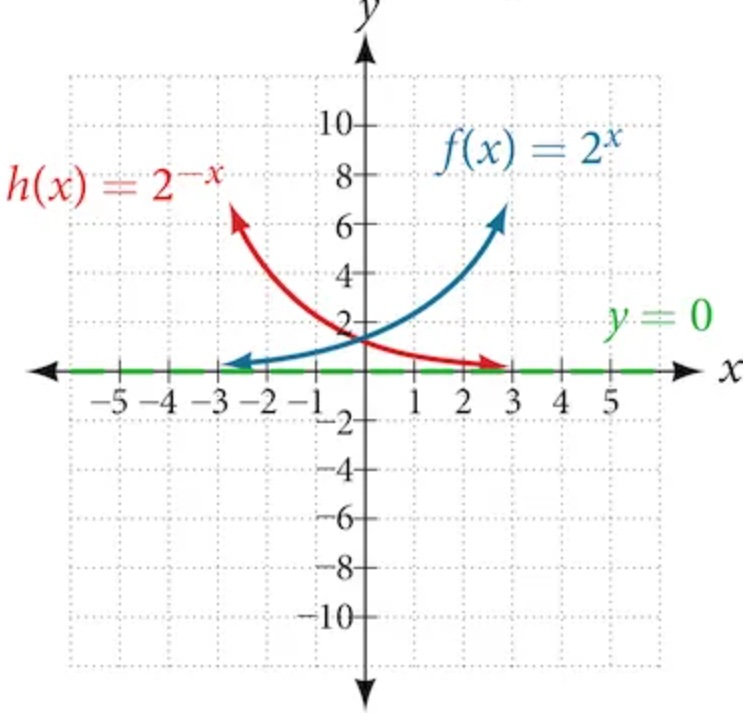
\includegraphics[width =2.8cm]{fig/exp2f.jpg}
\end{center}
\end{column}
\end{columns}

\end{frame}


\section{Trigonometry}



\begin{frame}\frametitle{Algebraic Functions}
\begin{columns}
\begin{column}{4.5cm}
An algebraic function provides a "y-value" for every "x-value"
\begin{itemize}
\item Linear: $y = x + 2$
\item Quadratic: $y = x^2$
\item Periodic: $y = sin(x)$
\end{itemize}
\end{column}
\begin{column}{7cm}
\begin{center}
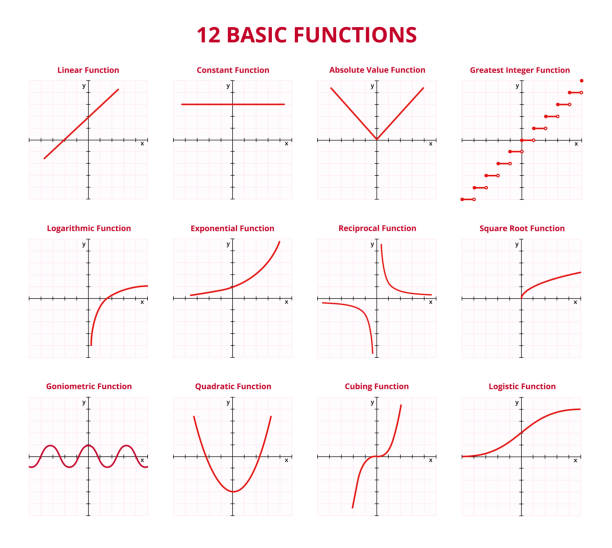
\includegraphics[width=7cm]{fig/basicfun.jpg}
\end{center}
\end{column}
\end{columns}
\end{frame}

\begin{frame}\frametitle{More Desmos Fun}

\begin{center}
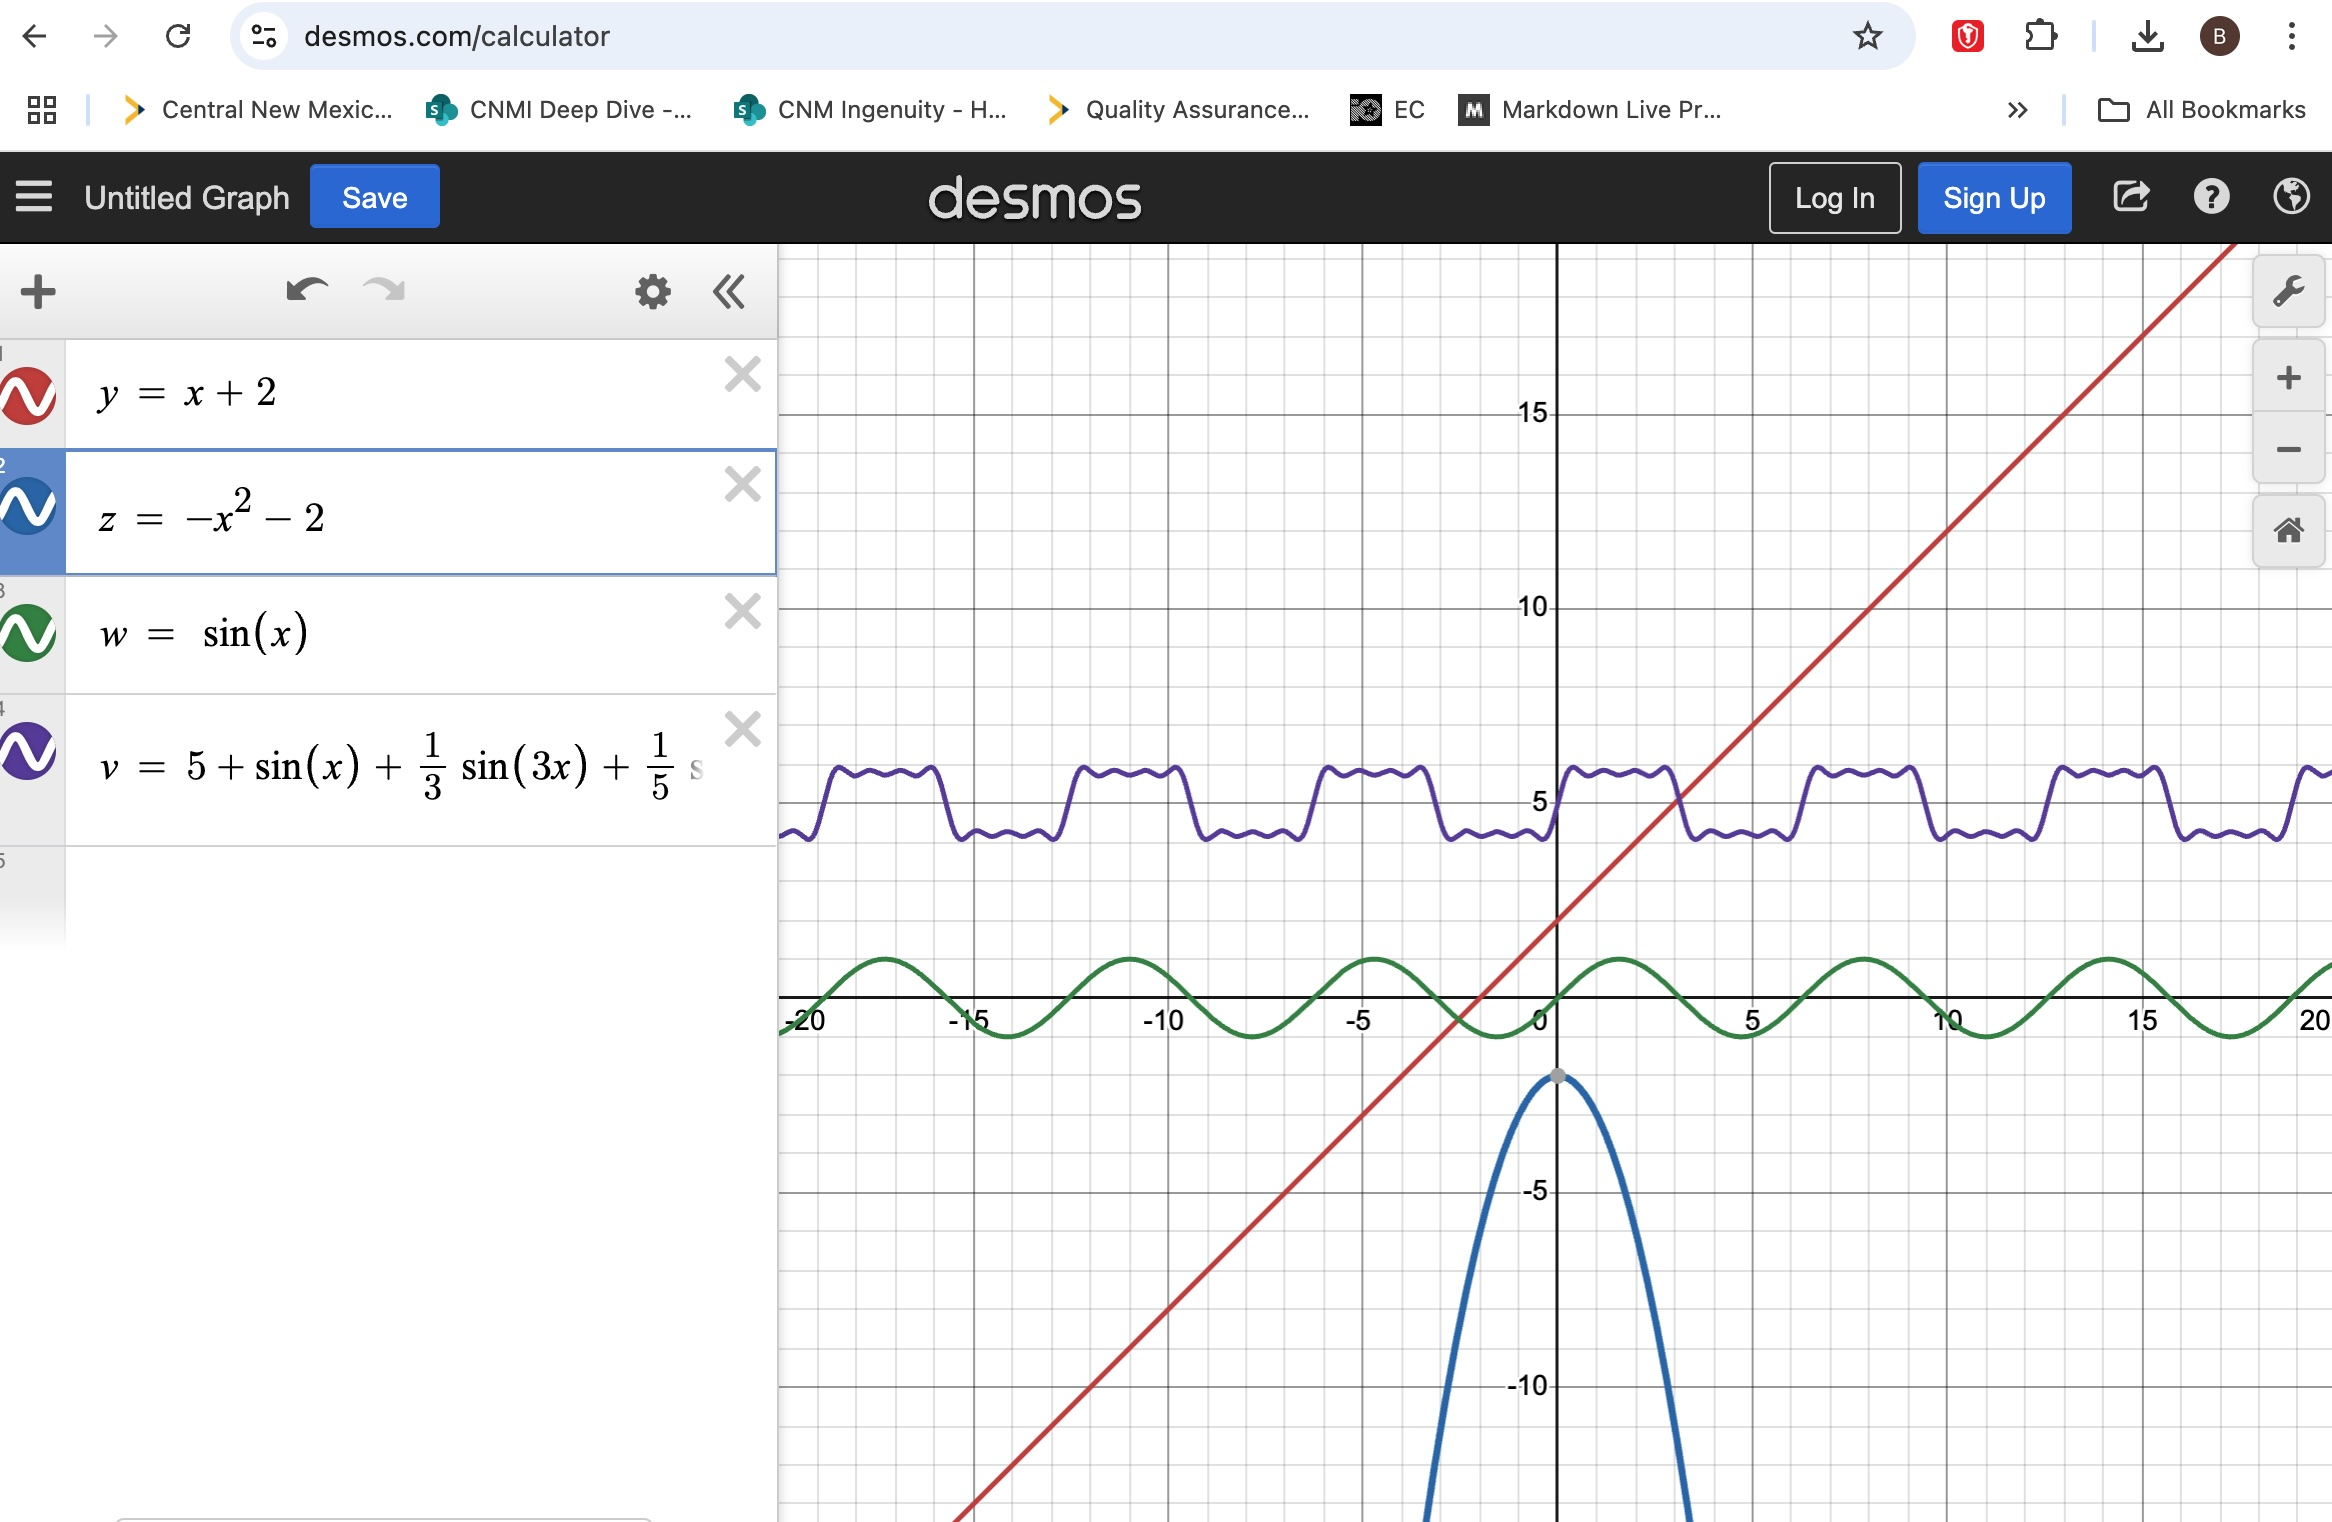
\includegraphics[width=12cm]{fig/desmosfun.jpg}
\end{center}
\end{frame}


\begin{frame}\frametitle{Pi ($\pi)$}

\begin{center}
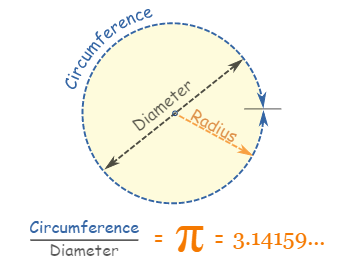
\includegraphics[width=8cm]{fig/pi.png}
\end{center}

\end{frame}


\begin{frame}\frametitle{Unit Circle and Trigonometric Functions}
The Unit Circle is a circle with a radius of 1.
\begin{columns}
\begin{column}{6cm}
\begin{center}
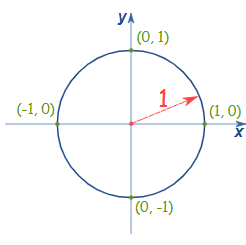
\includegraphics[scale=0.75]{fig/unitcircle.png}
\end{center}
\end{column}
\begin{column}{6cm}
\begin{center}
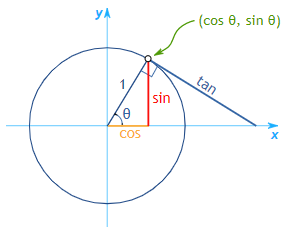
\includegraphics[scale=0.75]{fig/unitcircle_cst.png}
\end{center}
\end{column}
\end{columns}
The Unit Circle can be used to map out the trigonometric values of sine, cosine, and tangent.
\end{frame}


\begin{frame}\frametitle{Unit Circle and the Value of $sin(\theta)$}
\begin{columns}
\begin{column}{6cm}
\begin{center}
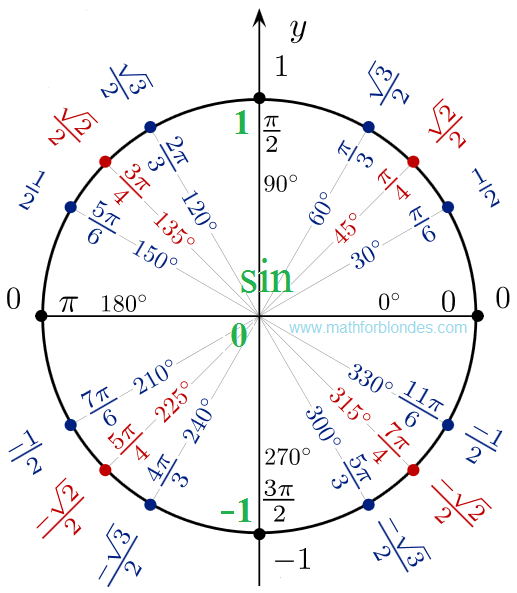
\includegraphics[scale=0.25]{fig/unitcircle_sin.png}
\end{center}
\end{column}
\begin{column}{6cm}
\begin{center}
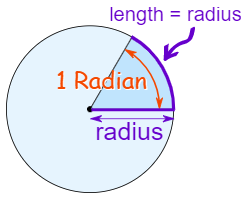
\includegraphics[scale=0.75]{fig/unitcircle_rad.png}
\end{center}
\end{column}
\end{columns}

\vspace{0.25cm}

\begin{itemize}
\item $sin(\theta)$ is the y-value of the point on the Unit Circle at angle $\theta$. 
\item In our trig functions, $\theta$ is measured in radians (rad), not degrees.
\item 360 degrees = $2 \pi$ radians.
\end{itemize}
\end{frame}



\begin{frame}\frametitle{Sine Waves}
\begin{center}
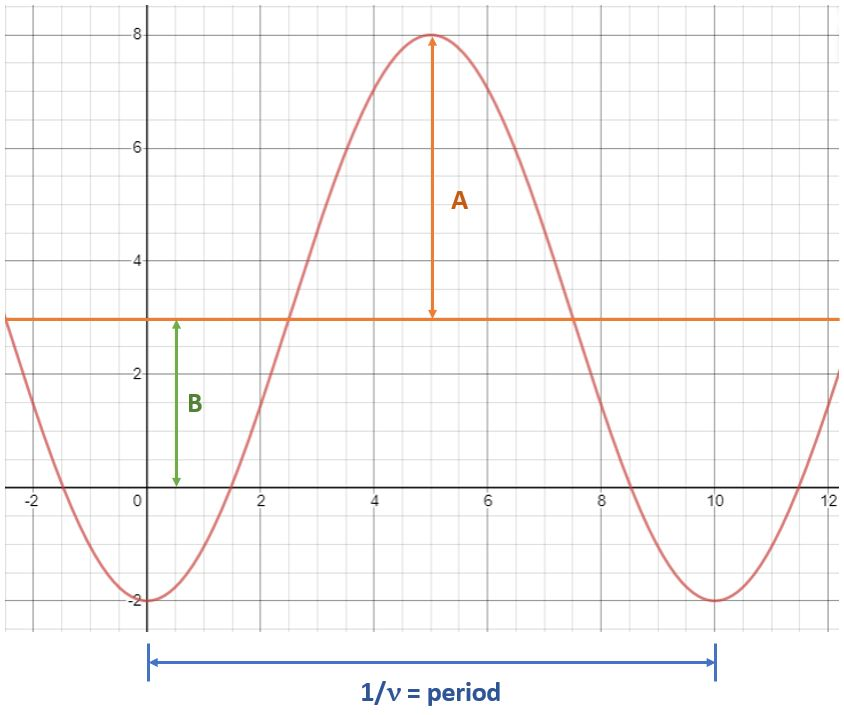
\includegraphics[scale=0.25]{fig/sin.jpg}
\end{center}

\begin{center}
$y = A * sin(2*\pi*\nu*t) + B$
\end{center}

where A = amplitude, B = offset, $\nu$ = frequency = $\frac{1}{period}$, 

and t = time in seconds.
\end{frame}


\begin{frame}\frametitle{Using Desmos (desmos.com/calculator)}
\begin{center}
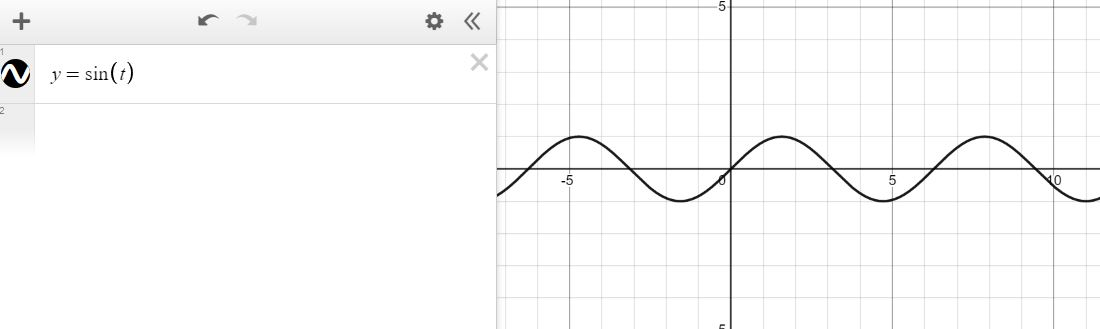
\includegraphics[scale=0.35]{fig/desmos1.jpg}
\end{center}
\begin{center}

\vspace{0.5cm}

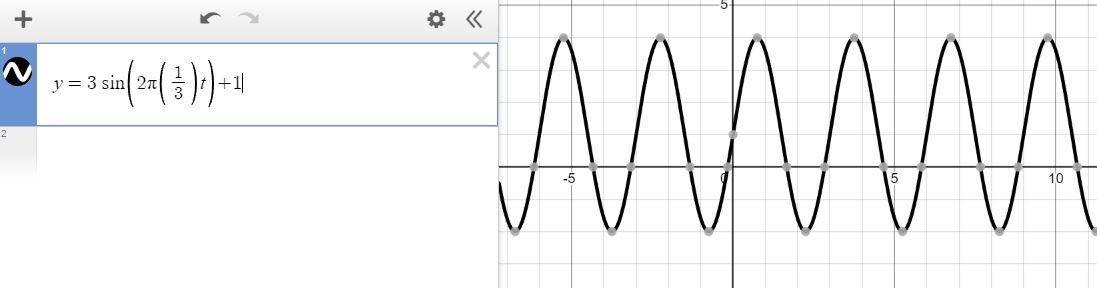
\includegraphics[scale=0.35]{fig/desmos2.jpg}
\end{center}
\end{frame}

\begin{frame}\frametitle{Phase Shift}
The sine wave can be shifted relative to each other by adding in a phase shift ($\phi$), which will shift the wave to the left or right.

Blue lags Red: 
\begin{center}
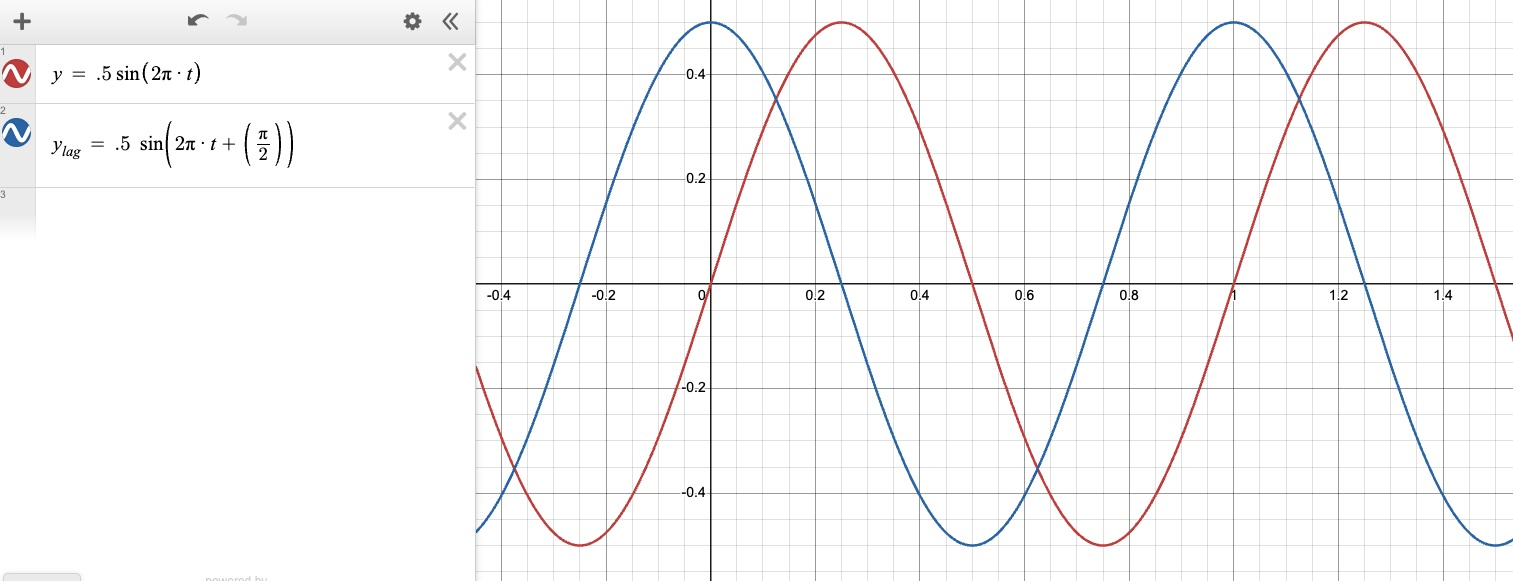
\includegraphics[height=2.6cm]{fig/sin_lag.jpg}
\end{center}

Green leads Red: 
\begin{center}
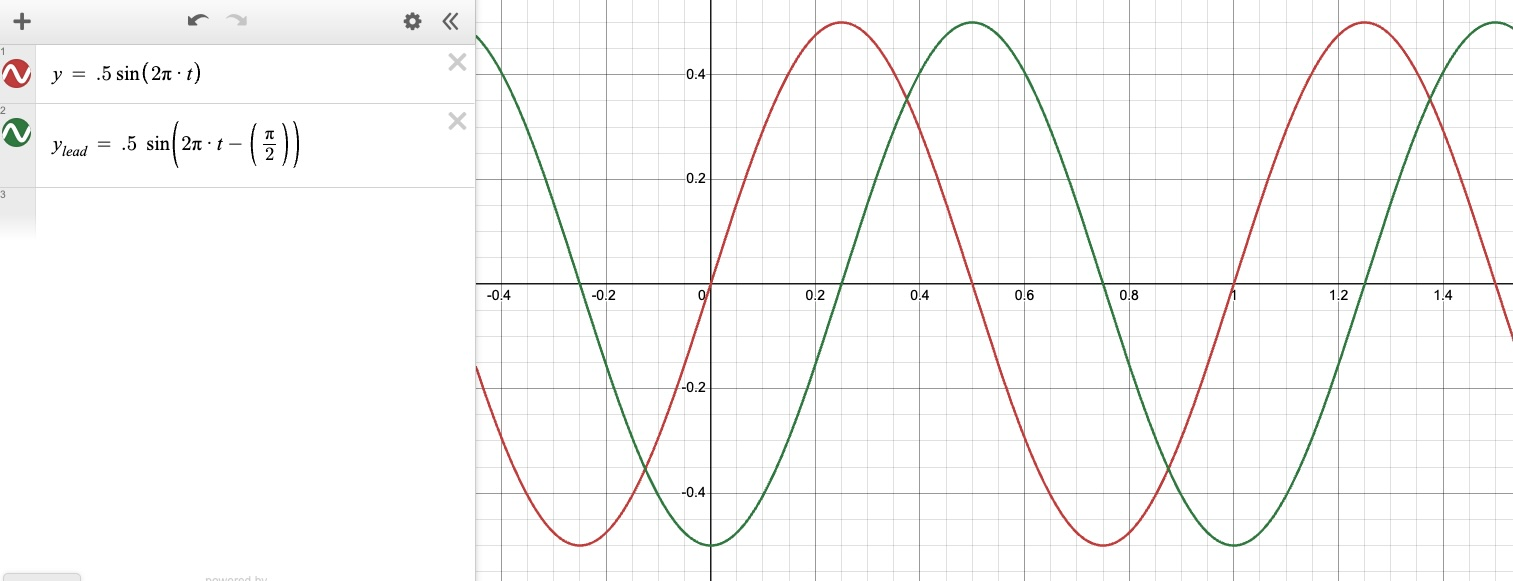
\includegraphics[height=2.6cm]{fig/sin_lead.jpg}
\end{center}

\end{frame}




\begin{frame}\frametitle{SOH CAH TOA}

\begin{itemize}
\item sin = opposite over hypotenuse
\item cos = adjacent over hypotenuse
\item tan = opposite over adjacent
\end{itemize}

\vspace{0.25cm}

\begin{center}
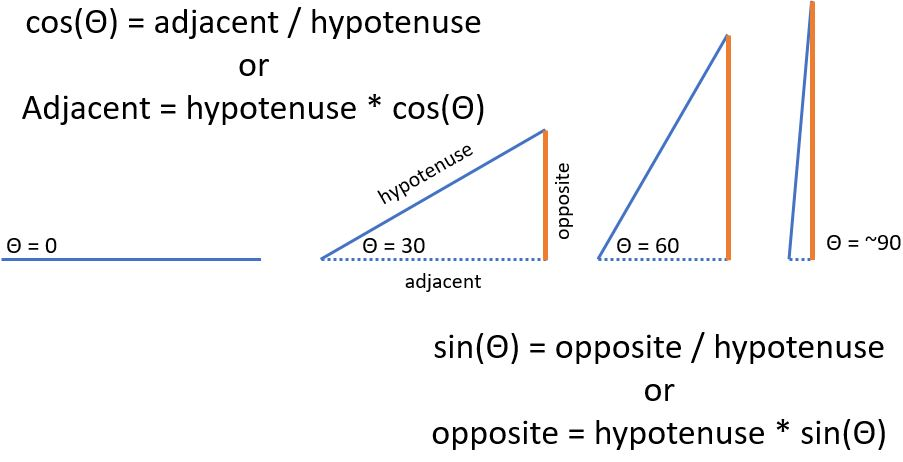
\includegraphics[scale=0.35]{fig/sohcahtoa.jpg}
\end{center}
\end{frame}

\section{Vectors}

\begin{frame}\frametitle{Scalars and Vectors}
Scalars are quantities that are fully described by a magnitude (or numerical value) alone.

Vectors are quantities that are fully described by both a magnitude and a direction.

\vspace{0.25cm}
\begin{center}
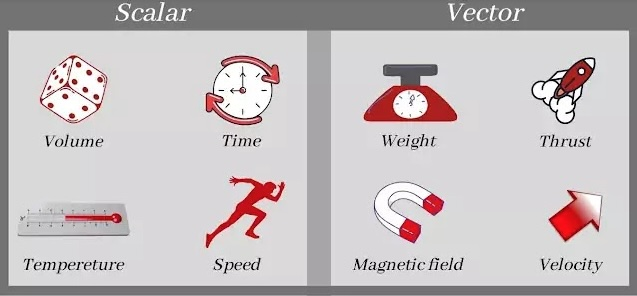
\includegraphics[width=8cm]{fig/scalarVector.jpg}
\end{center}
\end{frame}


\begin{frame}\frametitle{Vector Components}
\begin{columns}
\begin{column}{6cm}
Finding the components of a vector involves forming a right triangle and using trigonometry's SOH-CAH-TOA
\begin{itemize}
\item $A_x = A cos(\theta)$
\item $A_y = A sin(\theta)$
\end{itemize}
\end{column}
\begin{column}{5cm}

\begin{center}
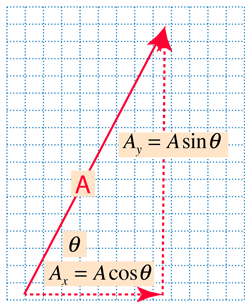
\includegraphics[width=4.8cm]{fig/vec5.png}
\end{center}
\end{column}
\end{columns}
\end{frame}


\begin{frame}\frametitle{Graphical Vector Addition}
\begin{columns}
\begin{column}{6cm}
Adding two vectors A and B graphically can be visualized like two successive walks, with the vector sum being the vector distance from the beginning to the end point. Representing the vectors by arrows drawn to scale, the beginning of vector B is placed at the end of vector A. The vector sum R can be drawn as the vector from the beginning to the end point.
\end{column}
\begin{column}{5cm}

\begin{center}
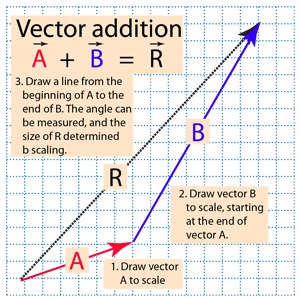
\includegraphics[width=4.8cm]{fig/vec1.png}
\end{center}
\end{column}
\end{columns}
\end{frame}


\begin{frame}\frametitle{Vector Components}
\begin{columns}
\begin{column}{6cm}
Finding the components of a vector involves forming a right triangle and using trigonometry's SOH-CAH-TOA
\begin{itemize}
\item Add the X components
\begin{itemize}
\item $A_x = 12 cos(20^\circ) = 11.3$
\item $B_x = 25 cos(60^\circ) = 12.5$
\item $R_x = A_x + B_x = 23.8$
\end{itemize}
\item Add the Y components
\begin{itemize}
\item $A_y = 12 sin(20^\circ) = 4.1$
\item $B_y = 25 sin(60^\circ) = 21.7$
\item $R_y = A_y + B_y = 25.8$
\end{itemize}
\end{itemize}
\end{column}
\begin{column}{5cm}

\begin{center}
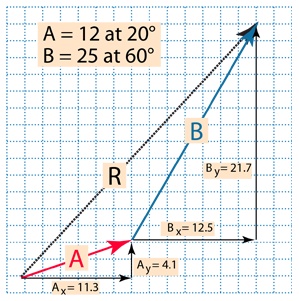
\includegraphics[width=4.8cm]{fig/vec2a.png}
\end{center}
\end{column}
\end{columns}
\end{frame}

\begin{frame}\frametitle{Polar Form}
\begin{columns}
\begin{column}{6cm}
After finding the components, the result can be placed in Polar Form:
\begin{itemize}
\item $R_x = 23.8$
\item $R_y = 25.8$
\item $R = \sqrt{R_x^2 + R_y^2} = 35.05$
\item $\theta_R = tan^{-1} (\frac{R-y}{R_x}) = 47.3^{\circ}$
\end{itemize}
\end{column}
\begin{column}{5cm}

\begin{center}
\includegraphics[width=4.8cm]{fig/vec4a.png}
\end{center}
\end{column}
\end{columns}
\end{frame}

\begin{frame}\frametitle{Unit Vectors in 3 Dimensions}
\begin{columns}
\begin{column}{6cm}
Vectors of unit length (i.e., length equals 1) can be used to specify the direction of vector quantities in various coordinate systems.

In Cartesian coordinates, it is typical to use i, j, and k to represent the unit vectors in the x, y, and z directions, respectively: 

\begin{equation}
\vec{r} = x \vec{i} + y \vec{j} + z \vec{k}
\end{equation}
\end{column}
\begin{column}{5cm}

\begin{center}
\includegraphics[width=4.8cm]{fig/uvec.jpg}
\end{center}
\end{column}
\end{columns}
\end{frame}

\begin{frame}\frametitle{Dot (Scalar) Product}
\begin{columns}
\begin{column}{6cm}
The dot (or inner or scalar) product of two vectors can be constructed by taking the component of the first vector in the direction  of the second vector and by multiplying it by the second vector's magnitude.

\begin{equation}
\vec{A} \cdot \vec{B} = AB cos(\theta)
\end{equation}

or

\begin{equation}
\vec{A} \cdot \vec{B} = A_x B_x + A_y B_y + A_z B_y
\end{equation}
\end{column}
\begin{column}{5cm}

\begin{center}
\includegraphics[width=4.8cm]{fig/vecdot.jpg}
\end{center}
\end{column}
\end{columns}
\end{frame}

\begin{frame}\frametitle{Cross (Vector) Product}
\begin{columns}
\begin{column}{6cm}
The magnitude of the cross (or outer or vector) product of vectors can be constructed by taking the product of the magnitude of the vectors times the sine of the angle between them.
\begin{equation}
\vec{A} \times \vec{B}_{magnitude} = AB sin(\theta)
\end{equation}

and the direction is given by the right hand rule.

\end{column}
\begin{column}{5cm}

\begin{center}
\includegraphics[width=4.8cm]{fig/veccross.jpg}

\includegraphics[width=2.8cm]{fig/righthandrule.png}
\end{center}
\end{column}
\end{columns}
In terms of unit vectors:

\begin{equation}
\vec{A} \times \vec{B} = \vec{i}(A_yB_z-A_zB_y) + \vec{j}(A_zB_x-A_xB_z) + \vec{k}(A_xB_y-A_yB_x)
\end{equation}
\end{frame}


\begin{frame}\frametitle{Bonus - Cross Product - Determinant Form}

THe cross product can be compactly stated in teh form of a determinant:

\[
\vec{A} \times \vec{B} =
\begin{vmatrix}
\vec{i} & \vec{j} & \vec{k} \\
A_x & A_y & A_z \\
B_x & B_y & B_z
\end{vmatrix}
\]

Which can be expanded to

\[
\vec{A} \times \vec{B} = \vec{i}(A_yB_z-A_zB_y) + \vec{j}(A_zB_x-A_xB_z) + \vec{k}(A_xB_y-A_yB_x)
\]
\end{frame}




\begin{frame}\frametitle{Pythagorean Theorem in 3 Dimensions}
\begin{columns}
\begin{column}{5cm}
\begin{center}
\includegraphics[width=5cm]{fig/pathagorean.png}

\vspace{0.25cm}

\includegraphics[width=4cm]{fig/pathag3D.jpg}

\end{center}
\end{column}
\begin{column}{5cm}
To add orthogonal (at right angles to each other) vectors in 3 Dimensions:
\begin{itemize}
\item $C = \sqrt{A_x^2 + A_y^2}$
\item $A_{total} = \sqrt{C^2 + A_z^2}$
\item $A_{total} = \sqrt{A_x^2 + A_y^2 + A_z^2}$
\end{itemize}
\end{column}
\end{columns}
\end{frame}

\section{Probability and Statistics}

\begin{frame}\frametitle{Statistics}
\begin{columns}
\begin{column}{5cm}
\begin{center}
\includegraphics[width=5cm]{fig/cartoonguidestats.jpg}
\end{center}
\end{column}
\begin{column}{5cm}
\begin{itemize}
\item Data Analysis: The gathering, display, and summary of data
\item Probability: The laws of chance (inside and outside of a casino)
\item Statistical Inference: the science of drawing statistical conclusions from specific data using the laws of probability
\end{itemize}
\end{column}
\end{columns}
\end{frame}

\begin{frame}\frametitle{Summary Statistics}
\begin{itemize}
\item Mean
\item Median
\item Spread
\item Interquartile Range (IQR)
\item Standard Deviation
\end{itemize}
\end{frame}


\end{document}
